% !TEX root = ../Masterarbeit.tex
\chapter{Grundlagen \& Begriffsbestimmung}
In diesem Kaptiel werden die Grundlagen geschaffen, auf jene der Hauptteil aufbaut. Zudem behandelt das Kapitel die Begriffsbestimmung und die genauen Eigenschaften reaktiver Systeme.\\
Da die Umsetzung reaktiver Systeme gewisse Programmierparadigmen vorausgesetzt, werden diese nach den reaktiven Merkmalen erklärt.

\section{Eigenschaften reaktiver Systeme}
Reaktive Anwendungen haben die Eigenschaften folgendes zu leisten bzw. foldenge Punkte zu erfüllen~\cite[S.~19ff]{kuhn_reactive_2015}~\cite[S.~6]{vernon_reactive_2016}.\\

\textbf{Eine reaktive Anwendung muss\ldots}
\begin{enumerate}
\item \ldots \textbf{auf variable Belastung reagieren (siehe~\ref{subsec:elastic}.).} Das System ist automatisch in der Lage dynamische Skalierung durchzuführen und nicht benötigte Ressourcen wieder freizugeben.
\item \ldots \textbf{auf Fehler reagieren (siehe~\ref{subsec:resilient}).} Die Software ist von Grund auf widerständsfähig gegenüber Fehlerzuständen. Die Wiederherstellung des Normalzustand erfolgt automatisch.
\item \ldots \textbf{auf Nutzer oder Komponenten reagieren (siehe~\ref{subsec:responsive}).} Jede Anfrage wird in der geforderte Antwortzeit bearbeitet und übertrifft diese eventuell sogar.
\item \ldots \textbf{auf Nachrichten reagieren (siehe~\ref{subsec:messagedriven}).} Das System verwendet asynchrone Nachrichtenübermittlung zwischen den Komponenten und ist somit \textit{message-driven}.
\end{enumerate}

Die nachfolgenden Abschnitte erklären die Merkmale im Detail und zeigen den Zusammenhang zwischen ihnen.

\subsection{Elastic}\label{subsec:elastic}
Eine reaktive Anwendung muss auf variable Belastung ebenso variable bzw. dynamisch reagieren können. Wird Beispielsweise ein Online Shop in einer Fernsehwerbung oder von einem bekannten Blog erwährt, müssen kurzfristig sehr viele Anfragen angemessen und zufriedenstellend verarbeitet werden~\cite[S.~39]{kuhn_reactive_2015}.\\
Um die gewünschten und geforderten Antwortzeiten einzuhalten, muss das System skalieren. Traditionellerweise ist hiermit \enquote{Scaling up} gemeint. Aufgrund der heutigen Anforderungen stößt man schnell an die Grenzen eines einzelen Hosts. Dementsprechend muss das System nicht nur vertikal sondern auch horizontal skalieren. Dazu muss das System auf mehrere Nodes verteilt werden~\cite[S.~7]{vernon_reactive_2016}. Es ist deshalb wichtig, die Teilaufgaben eines Systems zu identifizieren und auf einzelne Komponenten aufzuteilen, die dann wie bereits erwähnt auf einzelne Nodes verteilt werden können~\cite[S.~40]{kuhn_reactive_2015}.\\
Das Reactive Manifesto fordert zudem auch, das System so zu gestalten, dass es \enquote{Scaling down} fähig ist. Das bedeutet ungenutze und nicht benötigte Ressourcen müssen wieder freigegeben werden. Dadurch kann man ein hochskalierbares reaktives System kosteneffizient betreiben. Im Reactive Manifesto hat man sich auf den Begriff \textit{elastic} geeinigt, um deutlich zu machen, dass man in beide Richtungen skalieren kann. Bei reaktiven Applikationen kann spricht man deshalb von elastischer bzw. dymanischer Skalierung~\cite[S.~8]{vernon_reactive_2016}. Für die Software bedeutet dies, dass einzelne Nodes jederzeit hinzugefügt und entfernt werden können. Als Folge dessen muss das System \textit{location transparent} sein. Insofern dürfen dessen Komponenten und Funktionen nicht abhängig von einem Host sein~\cite[S.~8]{vernon_reactive_2016}. 

% TODO Little's Law
% TODO Infrastructure as a Service oder Cloud Computing; Enterprise IT OpenStack

\pagebreak

\subsection{Resilient}\label{subsec:resilient}
Eine Software \textit{resilient} (dt. widerstandsfähig) zu entwickeln bedeutet nicht, dass die Software fehlerfrei ist. Es bedeutet, dass die Software sich von einem Fehlerzustand erholen kann~\cite[S.~6]{vernon_reactive_2016}.\\
Man versucht bei dem Entwurf der Software Fehler von vornherein zu bedenken und mit ihnen sinnvoll umzugehen. Folgendes Zitat von Jonas Bonér macht deutlich, wie wichtig die Widerstandsfähigkeit einer Software ist.

\begin{quotation}
Without resilience, nothing else matters. If your beautiful, production-grade, elastic, scalable, highly concurrent, non-blocking, asynchronous, highly responsive and performant application isn't running, then you're back to square one. It starts and ends with resilience.~\citetext{Bonér, Jonas; 2015}
\end{quotation}

Im Grunde ist diese Aussage trivial. Eine Software die nicht läuft, ist unbrauchbar --- egal wie komplex und durchdacht die Architektur auch sein mag.\\
Es ist aber nicht nur die eigene Software die betroffen sein kann. Andere externe Softwarekomponenten von denen man abhängt oder auch die Hardware kann im laufenden Betrieb Probleme bereiten~\cite[S.~33]{kuhn_reactive_2015}.\\
Der Schluss, den man daraus ziehen sollte, lautet deshalb nicht, ob ein Fehler auftritt sondern viel mehr wann und wie häufig das passiert. Für den Benutzer ist es nebensächlich warum ein interner Fehler aufgetreten ist. Die Anwendung wird in diesem Moment nicht das tun, was der Benutzer von ihr erwartet~\cite[S.~33]{kuhn_reactive_2015}.\\

Im Reactive Manifesto hat man für dieses Problem bzw. die Eigenschaft ganz bewusst den Begriff \textit{resilience} und nicht \textit{reliability} (dt. Ausfallsicherheit) gewählt. Man möchte deutlich machen, dass es nahezu unmöglich ist, ein ausfallsicheres System zu schaffen. Deshalb setzt man auf widerstandsfähige Systeme, welche mit Fehlerzuständen sinnvoll umgehen und vorallem sich von dieses wieder erholen. Folglich ist ein reaktives System nicht nur \textit{fault tolerant} (dt. Fehler tolerant) sondern geht noch einen Schritt weiter~\cite[S.~34]{kuhn_reactive_2015}.\\

Um die Eigenschaft \textit{resilience} zu erfüllen, muss das System in Komponenten aufgeteilt und anschließend verteilen (engl. distribute) werden. Zusätzlich ist es nötwendig die verteilen Komponenten von einander abzuschotten (engl. compartmentalize)~\cite[S.~34]{kuhn_reactive_2015}~\cite[S.~7]{vernon_reactive_2016}.\\
Aufgrund der verteilten und abgeschottenten Komponenten können Fehler isoliert werden. Hierfür führt man das Prinzip der \textit{supervisor} ein. Nach- bzw. untergeordnete Komponenten informieren ihren \textit{supervisor} im Falle eines Fehlers. Dieser hat nun die Möglichkeit die Subkomponente z.B. neuzustarten oder eine erneute Anfrage zustellen. 

\subsection{Responsive}\label{subsec:responsive}
Eine reaktive Anwendung muss zu jederzeit auf jede Anfragen reagieren. Das heißt die Anwendung ist jederzeit \textit{responsive} (dt. antwortbereit). Anfragen können nicht nur durch einen Benutzer ausgelöst werden, sondern können auch von anderen Diensten oder Komponenten initiert werden. Als Client einer reaktiven Anwendung muss man sich drauf verlassen können, dass eine Antwort in einem festgelegten Zeitraum eintrifft. Das bedeutet es müssen \textit{timeouts} festgelegt werden, nachdem eine Anfrage für fehlerhaft erklärt wird.\\
(Außerdem muss eine reaktive Anwendung Anfragen nebenläufig und parallel bearbeiten.)
Ist eine Anwendung nicht \textit{elastic} (siehe~\ref{subsec:elastic}) und/oder nicht \textit{resilient} (siehe~\ref{subsec:resilient}) kann sie auch nicht \textit{responsive} sein. Eine reaktive Anwendung muss unter Last skalieren, um die geforderte maximale Antwortzeit einzuhalten oder zu vermeiden, dass das System gar ganz ausfällt. Fallen Komponenten aus, z.B. durch einen unvorhergesehenen Hardwarefehler, könnten diese aufgrund der \textit{location transparency} auf einem anderen Node neugestartet werden.

\pagebreak

\subsection{Message-driven}\label{subsec:messagedriven}
Um die bereits erwähnten Eigenschaften \textit{elasticity} (\ref{subsec:elastic}), \textit{resilience} (\ref{subsec:resilient}) sowie die daraus folgende \textit{responsiveness} (\ref{subsec:responsive}) zu erfüllen, müssen reaktive Anwendungen \textit{message-driven} sein~\cite{webber_what_2014}~\cite[S.~43]{kuhn_reactive_2015}. Somit ist die Basis einer reaktiven Anwendung die vierte Eigenschaft aus dem Reactive Manifesto~\cite{boner_reactive_2014}.\\
Ist ein System \textit{message-driven} erfolgt die Kommunikation ausschließlich über asynchronen Nachrichtenaustausch zwischen den Komponenten, wodurch eine strikte Abgrenzung der Komponenten erfolgt. Durch die Abstraktion der Kommunikation wird eine lose Kopplung zwischen den Komponenten sichergestellt. Darüber hinaus sind die Komponenten voneinander isoliert, wodurch es möglich ist, Fehler als Nachrichten zu delegieren (siehe~\ref{subsec:resilient}).\\
Durch den expliziten Nachrichtenaustausch kann über \textit{message queues} und \textit{flow control} die Last verteilt und kontrolliert werden. Ebenso wird die gewünschte \textit{location transparency} durch die Entkopplung über den asynchronen Nachrichtenaustausch ermöglicht~\cite{boner_reactive_2015}~\cite[S.~43]{kuhn_reactive_2015}.\\
Die folgende Abbildung (Abb. \ref{fig:four-traits}) sollen den Zusammenhang der vier Merkmale nochmals verdeutlichen. Neben dem wohl wichtigesten Ziel (\textit{responsive}) hat die reaktive Architektur den Vorteil ebenso wartbare wie auch erweiterbare Anwendungen zu schaffen. Jedoch werde die weiteren Ziele nur in der Einleitung des Reactive Manifestos und nicht als Kerneigenschaft formuliert~\cite{boner_reactive_2014}. Die Ziele ereicht man durch die Eigenschaften \textit{elasticity} und \textit{resilience}. Das Grundgerust von alle dem ist die asynchrone, nicht-blockierende und Nachrichtengetriebene Kommunikation (\textit{message-driven}).

\begin{figure}[H]
 \centering
 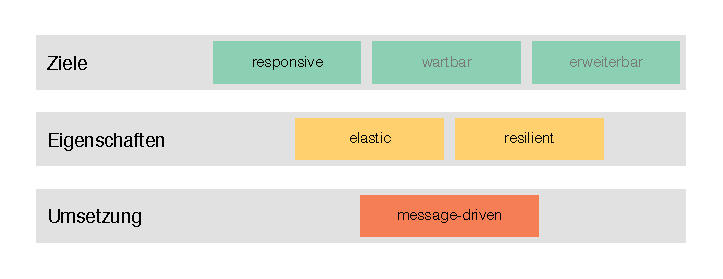
\includegraphics[width=1.0\textwidth]{3-Grundlagen/four-traits/four-traits.eps}
 \caption{Die vier Merkmale einer reaktiven Anwendung \cite{kuhn_code_2015}}
 \label{fig:four-traits}
\end{figure}

\pagebreak

\section{Parallelität und Nebenläufigkeit}


We need to bring distributed computing down to the level of CPUs, because latency will be always a problem. Moore's Law. To speed up you can't wait for faster CPUs anymore, you need to scale on multiple CPUs.

% Non-blocking communication allows recipients to only consume resources while active, leading to more efficient system utilization. 

% communicate to share information, don't share information to communicate
% Conclusion reactive systems are distributed


\subsection{Share nothing}
Decoupling and single responsibility principle will result in clear boundaries.\\
Share memory to communicate.\\
Communicate to share memory.
% TODO Decoupling
% Single responsibility principle
% Containment of failure, implementation details & responsibility
% Share nothing -> clear boundaries
% TODO responsiveness in synchronous systems
% TODO Waldo et al "A Note on Distributed Computing"
% TODO Peter Deutsch Distributed Systems

% TODO solution for this: reactive manifesto & actor model


\section{Functional programming}
% Non-determinism caused by concurrent threads accessing shared mutable state. To get determinism, avoid mutable state. To avoid mutable state it means to program functially.

\subsection{First-class functions}
\subsection{Immutable State}

\section{Reactive programming}
Reaktive Programmierung in der Entwicklung von Benutzeroberflächen üblich und verbreitet. Als Entwickler einer GUI stetig auf eingehende Events reagieren (z.B. Cursorbewegung, Tastendruck). Während der Verarbeitung dieser soll die Benutzeroberfläche nicht blockieren und Eingaben dadurch verhindern. Eine Benutzeroberfläche muss responsive sein, um den Benutzer nicht zu verärgern.

- Nachrichtenstorm
- Events: facts about things that have happend

\subsection{Reactive extensions \& Oberservable}
Reactive extensions are libraries for asynchronous and therefore reactive programming.
Evolution: imperative -> functional -> reactive
